En caso de que existan restricciones en secuencias permitidas
todav\'ia se puede obtener una ecuaci\'on diferencial de este tipo y
encontrar C de la ecuaci\'on caracter\'istica. En el caso mencionado
anteriormente de la telegraf\'ia
\begin{equation}
N(t) = N(t-2)+N(t-4)+N(t-5)+N(t-7)+N(t-8)+N(t-10),
\end{equation}
como se ve por el c\'alculo de secuencia de los s\'imbolos de acuerdo
al \'ultimo o al siguiente \'ultimo s\'imbolo ocurriendo.  Por lo
tanto $-\log\mu_{0}$ donde $\mu_{0}$ es la ra\'iz positiva de $1
= \mu^{2}+\mu^{4}+\mu^{5}+\mu^{7}+\mu^{8}+\mu^{10}$. Resoviendo eso
encontramos que $C = 0.539$.

Una restricci\'on general se puede colocar en secuencias como la
siguiente: Imagenemos un numero de estados posibles $a_{1},
a_{2},\ldots,{m}$. Por cada estado solo ciertos s\'imbolos del
conjunto $S_{1},\ldots,S_{n}$ pueden ser transmitidos (diferentes
subconjuntos por cada estado). Cuando uno de esos han sido
transmitidos el estado cambia a un nuevo estado dependiendo de el
viejo estado y del s\'imbolo en particular transmitido. Un ejemplo
simple de esto es el caso del tel\'egrafo. Hay dos estados en
funci\'on de si o no un espacio era el \'ultimo s\'imbolo transmtido.
Si es as\'i, entonces s\'olo un punto o una raya puede ser enviado al
lado y el estado cambia siempre. Si no, cualquier s\'imbolo puede ser
transmitido y los cambios de estado si un espacio es enviado, de lo
contrario sigue siendo el mismo.  Las condiciones pueden ser indicadas
en una gr\'afica lineal como se ve en la figura \ref{fig:2}. 

\begin{figure}[!ht]
\centerline{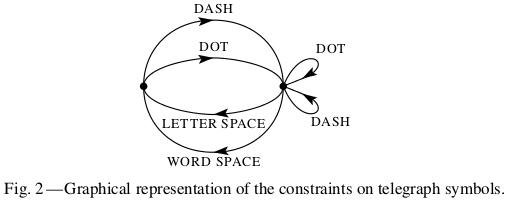
\includegraphics[width=120mm]{Imagenes/Pagina4-Figura2.png}}
\caption{Una representaci\'{o}n gr\'{a}fica de las restricciones 
en los s\'{\i}mbolos telegr\'{a}ficos.}
% FALTA CORTAR Y TRADUCIR LA GRAFICA
\label{fig:2}
\end{figure}

Los puntos de uni\'on correspoden a los estados y las l\'ineas
indicando los s\'imbolos posibles en un estado y el estado resultante.
En el Anexo \ref{a1} se muestran que si las condiciones en las
secuencias permitidas puede ser descrita en la forma $C$ puede existir
y se puede calcular de acuerdo con el siguiente resultado:
\begin{theorem}
 Siendo $b_{ij}^{(s)}$ la duraci\'on del $s$\'{e}simo s\'{\i}mbolo, el
cual es permisible en el estado $i$ y conduce al estado $j$. Despu\'es la
capacidad del canal $C$ es igual a $\log W$ donde $W$ es la ra\'iz real
m\'as grande de la ecuaci\'on:
\begin{equation}
\left|\sum_{s}W^{-b_{ij}^{(s)}}-\delta_{ij}\right|=0,
\end{equation}
donde $\delta_{ij}=1$ si $i=j$ y es cero en cualquier otro caso
\end{theorem}
Por ejemplo en el caso del tel\'egrafo el determinante es:
\begin{equation}
\begin{vmatrix}
-1&(W^{-2}+W^{-2}) \\ 
 (W^{-3}+W^{-6})&(W^{-2}+W^{-2}-1) 
\end{vmatrix}=0
\end{equation}
Esta expansi\'on conduce a la ecuaci\'on dada anteriormente para este
caso.

\clearpage

\chapter{La fuente discreta de la informaci\'on}
\label{sec:2}

Hemos visto que bajo condiciones muy generales el logaritmo del
n\'umero de se\~nales posibles en un canal discreto aumenta
linealmente con el tiempo. La capacidad de transmisi\'on de
informaci\'on se puede especificar dando a esta tasa de aumento, el
n\'umero de bits por segundo necesarios para especificar la se\~nal
particular utilizada.  

Consideremos ahora la fuente de
informaci\'on. {\textquestiondown}C\'omo es una fuente de
informaci\'on a ser descrita matem\'aticamente, y la cantidad de
informaci\'on en bits por segundo se produce en una fuente dada? El
principal punto en cuesti\'on es la efecto de los datos estad\'isticos
sobre la fuente en la reducci\'on de la capacidad requerida de la
canal, por el uso de una correcta codificaci\'on de la
informaci\'on. En la telegraf\'ia, por ejemplo, los mensajes para ser
transmitidos consisten en secuencias de letras. Estas secuencias, sin
embargo, no son completamente aleatorias.

En general, las oraciones tienen una estructura estad\'istica de, por
ejemplo, ingl\'es. La letra $E$ se produce con m\'as frecuencia que
$Q$, la secuencia $TH$ con m\'as frecuencia que $XP$, etc. La
existencia de esta estructura permite hacer un ahorro en el tiempo (o
capacidad de canal) para codificar correctamente las secuencias de
mensajes en una secuencia de se\~nales. Esto ya se hace en una medida
limitada en telegraf\'ia utilizando el s\'imbolo de canal m\'as corto,
un punto, por la m\'as letra E que es la m\'as com\'un en ingl\'es,
mientras que las letras infrecuentes, $Q$, $X$, $Z$ est\'an
representados por secuencias m\'as largas de puntos y rayas. Esta idea
se lleva a\'un m\'as lejos en ciertos c\'odigos comerciales donde las
palabras y frases comunes est\'an representados por cuatro o cinco
grupos de c\'odigo de letra con un considerable ahorro de tiempo
promedio.  Los telegramas est\'andar de saludo y aniversario se han
usado tanto hasta el punto de que se codifican una o dos frases en una
secuencia relativamente corta de n\'umeros.

Podemos pensar en una fuente discreta de generar el mensaje, s\'imbolo
por s\'imbolo. Se elegir\'a una sucesi\'on de s\'imbolos de acuerdo
con ciertas probabilidades dependiendo, en general, de las opciones
anteriores, as\'i como los s\'imbolos en cuesti\'on. Un sistema
f\'isico, o un modelo matem\'atico de un sistema que produce una
secuencia de s\'imbolos gobernadas por un conjunto de probabilidades,
se le conoce como un proceso estoc\'astico.  Podemos considerar por lo
tanto que una fuente discreta puede ser representada por un proceso
estoc\'astico. A la inversa, cualquier proceso estoc\'astico que
produce una secuencia discreta de s\'imbolos elegidos a partir de un
conjunto finito puede ser considerado una fuente discreta. Esto
incluye casos como:

\begin{enumerate}
\item{Lenguajes naturales escritos como el ingl\'es, alem\'an y chino.}

\item{Fuentes de informaci\'on continuos que se han vuelto discretas por
alg\'un proceso de cuantificaci\'on. Por ejemplo, la se\~nal de voz
cuantizada desde un transmisor PCM, o una se\~nal de televisi\'on
cuantizada.}

\item{Casos matem\'aticos en los que simplemente se definen abstractamente
procesos estoc\'asticos que generan una secuencia de s\'imbolos. Los
siguientes son ejemplos de este \'ultimo tipo de fuente.}
\end{enumerate}

\begin{exmp}
Supongamos que tenemos cinco letras $A$, $B$, $C$, $D$, $E$, que se
eligen cada una con probabilidad $0.2$, elecciones sucesivas siendo
independientes. Esto dar\'ia lugar a una secuencia, la siguiente es un
t\'ipico ejemplo:
$$B D C B C E C C C A D C B D D A A E C E E A,$$
$$A B B A E D E C A C E E E E B A C B C E A D.$$
Este fue construido con el uso de una tabla de azar.
\label{ej:a}
\end{exmp}

\begin{exmp}
Utilizando las mismas cinco letras y siendo las probabilidades $0.4$,
$0.1$, $0.2$, $0.2$, $0.1$, respectivamente, con decisiones independientes
sucesivas. Un mensaje t\'ipico de esta fuente es entonces:
$$A A A C D C B D C E A A D A D A C E D A,$$
$$E A D C A B E D A D E D C C A A A A A D.$$
\label{ej:b}
\end{exmp}

\begin{exmp}
Una estructura m\'as complicada se obtiene si los s\'imbolos no son
elegidos de manera independiente pero sus probabilidades dependen de
las letras anteriores. En el caso m\'as simple este tipo de elecci\'on
depende solamente de la letra anterior y no de las que estan antes. La
estructura estad\'istica puede entonces ser descrita por un conjunto
de probabilidades de transici\'on $p_{i}(j)$, la probabilidad de que
la letra $i$ es seguida por la letra $j$. Los \'indices de $i$ y $j$
se extienden sobre todos los s\'imbolos posibles. Una segunda manera
equivalente de especificar la estructura es dar el ``diagrama'' de
probabilidades $p(i,j)$, la frecuencia relativa de el diagrama $i j$.
La frecuencia de letras $p(i)$, (la probabilidad de la letra i), la
transici\'on de probabilidades $p_{i}(j)$ y el diagrama de
probabilidades $p(i,j)$ son descritos en las siguientes formulas:
\begin{equation}
p(i)=\sum_{j}p(i,j)=\sum_{j}p(j,i)=\sum_{j}p(j)p_{j}(i) 
\end{equation}

falta terminar ejemplo C.
\label{ej:c}
\end{exmp}


